\section{Runtime Representation of Terms}
\label{section:runtime-terms}

All runtime terms are represented as shown in the class diagram in Figure \ref{class-diagram-runtime-term}

\begin{figure}[H]
	\centering
	\makebox[\textwidth][c] { 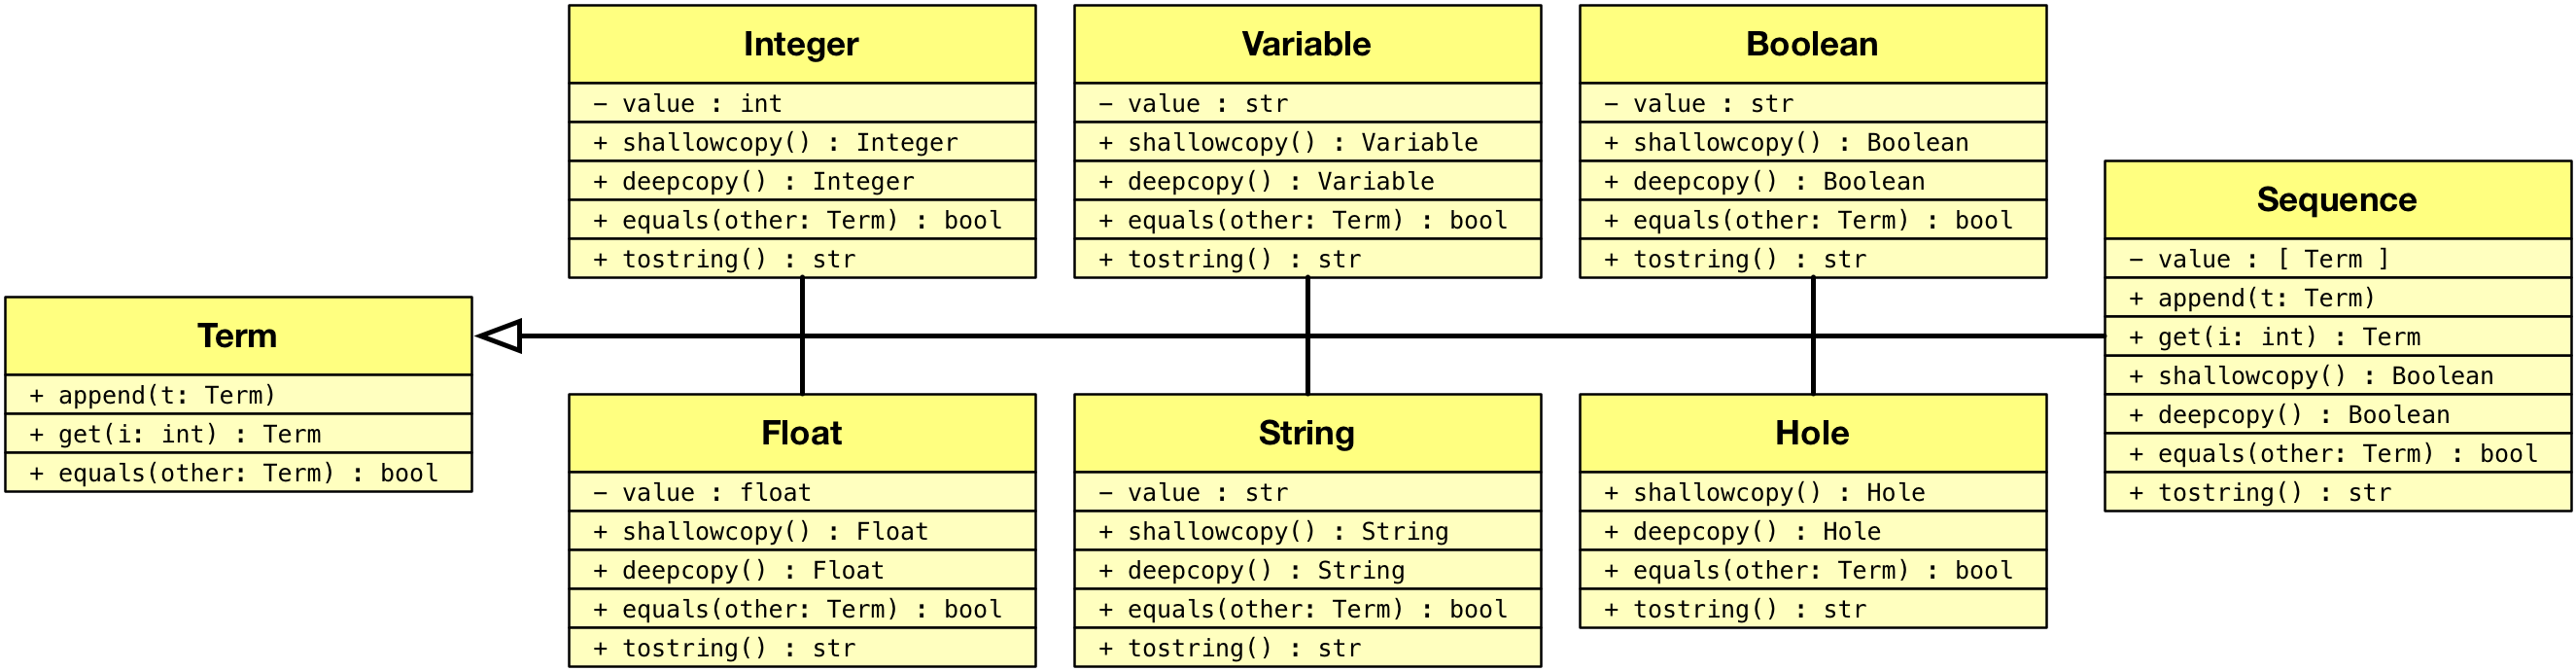
\includegraphics[scale=0.17]{class-diagram-runtime-term.png} }
\caption{\texttt{Term} class hierarchy.}
\label{class-diagram-runtime-term}
\end{figure}

These classes are all very similar and essentially just act as a wrapper for some primitive type. \texttt{Term} is the base class. Due to how RPython's type inference works creating a single class to represent all child classes such as \texttt{String} or \texttt{Float} results in the following compilation error.  Since the \texttt{LeafNode} instance is created with the \texttt{helloworld!} string, any other instantiation of \texttt{LeafNode} expects its second argument to be of type \texttt{string}. 

One may notice that, for example, \texttt{String} and \texttt{Variable} could be merged into one class and an additional \texttt{tag} field could be introduced to differentiate between strings and variables. However, since \texttt{isinstance} function is supported by RPython, such change would make term comparison logic more complex.

\begin{minted}[tabsize=2,obeytabs,fontsize=\normalsize]{python}
class LeafNode:
    def __init__(self, kind, value):
        self.kind = kind 
        self.value = value

def entrypoint():
    p = LeafNode('hello world!')
    q = LeafNode(12.5)

# UnionError:
#  SomeString(const='hello world!', no_nul=True)
#  SomeFloat(const=12.5)
\end{minted}

All classes implement the following methods.
\begin{itemize}
\item \texttt{shallow\_copy} returns an exact copy of the term. This kind of copying is not recursive.
\item
\texttt{deep\_copy} copies the term recursively. In practice, it duplicates \texttt{shallow\_copy} for every term type except \texttt{Sequence}; each term in the sequence is deep-copied and a new \texttt{Sequence} instance is returned containing copied terms.
\item
\texttt{equals} compares two terms based on the type of the term and then on the value.
\item
\texttt{tostring} returns a string representing the term. These are made to look like actual Racket expressions.
\end{itemize}
 
In addition, the following utility functions are provided to make implementation of certain functionalities easier.

\begin{itemize}
\item
	\texttt{copy\_path\_and\_replace\_last}. Given a path of terms $t_1, ..., t_n$  where terms $t_1, ..., t_{n-1}$ are expected to be of type \texttt{Sequence}, and given term $t_n^{\prime}$, the path is copied using \texttt{shallow\_copy} up to $t_n$, producing terms $t_1^\prime, ..., t_{n-1}^\prime$ and $t_n$ is replaced with $t_n^{\prime}$. All pointers to successor terms are also fixed up; that is, given two copied terms $t_i^{\prime}$ and $t_{i+1}^{\prime}$, $t_i^{\prime}$ will point to $t_{i+1}^{\prime}$ instead of $t_{i+1}$. $t_1^\prime$ is returned.
\item
	\texttt{locatehole} recursively traverses the term $t$ looking for term of type \texttt{Hole}. Each term on the path to \texttt{Hole} is recorded and upon successful search the path is returned.
\item
	\texttt{plughole}. Given two terms $t_1$ and $t_2$, first \texttt{locatehole} is called with $t_1$ as an argument. If a resulting path is non-empty, the result of \texttt{copy\_path\_and\_replace\_last} called with resulting path and $t_2$ is returned. Otherwise, $t_1$ is returned.
\item
	\texttt{asserttermsequal}. Given two terms, \texttt{equals} method is called and an Exception is raised if \texttt{equals} returns False.
\item
	\texttt{asserttermlistsequal}. Given two lists $T_1$, $T_2$ containing \texttt{Term} instances, \\ \texttt{asserttermsequal} function is called for each pair $t_1 \in T_1$ and $t_2 \in T_2$. Both lists are expected to have same lengths.
\item 
	\texttt{asserttermsequalpairwise}. Given a list $T$ containing \texttt{Term} instances, asserts that each pair $t_i, t_{i+1} \in T$ is equal, using \texttt{equals} method described previously.
\end{itemize}
